\documentclass[12pt]{article}
\usepackage[margin=1in]{geometry}
\usepackage{amsmath}
\usepackage{hyperref}
\usepackage{graphicx}
\graphicspath{ {./} }


\title{A Comparative Analysis of Machine Learning Models for Predicting the Lorenz System}
\author{Rushi Chaudhary \\
Memorial University of Newfoundland \\
rrchaudhary@mun.ca}
\date{October 27, 2025}

\begin{document}

\maketitle

\section{Introduction}

The Lorenz system, introduced by Edward N. Lorenz in his seminal 1963 paper on deterministic nonperiodic flow, serves as a foundational model in the study of chaotic dynamics\cite{lorenz1963deterministic}. Originally derived as a simplified mathematical representation of atmospheric convection, the system consists of three coupled nonlinear ordinary differential equations:

\begin{align}
\dot{x} &= \sigma (y - x), \\
\dot{y} &= x (\rho - z) - y, \\
\dot{z} &= xy - \beta z,
\end{align}

where $x$, $y$, and $z$ represent variables related to convective motion, horizontal temperature variation, and vertical temperature variation, respectively. The parameters $\sigma$, $\rho$, and $\beta$ control the system's behavior. The Lorenz system exhibits chaotic attractors characterized by sensitive dependence on initial conditions—a phenomenon popularly known as the ``butterfly effect''\cite{gleick1987chaos}. This sensitivity implies that small changes in starting points can lead to vastly different trajectories, making long-term prediction inherently challenging despite the system's deterministic nature.

Chaotic systems like the Lorenz model are ubiquitous in natural phenomena, appearing in fields such as meteorology, fluid dynamics, and even biology. Traditional numerical methods for solving these ordinary differential equations (ODEs), such as Euler's method or higher-order Runge-Kutta integrators, provide reliable short-term forecasts but accumulate errors over time due to numerical instability and approximations. As a result, predicting the long-term behavior of such systems requires innovative approaches that can capture underlying patterns while mitigating error propagation.

In recent decades, machine learning (ML) has emerged as a powerful tool for modeling and forecasting complex dynamical systems. Unlike traditional methods that rely on explicit integration of known equations, ML techniques can learn directly from data, identifying hidden structures in time-series observations. For chaotic systems, recurrent neural networks (RNNs), particularly Long Short-Term Memory (LSTM) architectures, have shown promise in handling sequential data and capturing temporal dependencies\cite{dubois2020data}. These models excel in short-term predictions by learning from historical trajectories but may struggle with long-term stability due to the amplification of small errors in chaotic regimes.

To address these limitations, physics-informed approaches integrate domain knowledge into ML frameworks. Physics-Informed Neural Networks (PINNs), for instance, embed the governing differential equations into the loss function, ensuring that predictions adhere to physical laws while fitting the data. Related scientific ML methods, such as Neural Ordinary Differential Equations (Neural ODEs) and Universal Differential Equations (UDEs), model the derivative functions themselves using neural networks, offering interpretable and efficient alternatives for simulating ODE systems\cite{kashyap2024modeling}. These hybrid techniques combine the flexibility of data-driven learning with the robustness of physical constraints, potentially yielding superior performance in chaotic environments.

This project undertakes a comparative analysis of various ML models—regression, LSTMs, and PINNs—for predicting the evolution of the Lorenz system. The primary goal is to assess their efficacy in both short-term and long-term forecasting horizons, quantified through metrics such as mean squared error (MSE) and root mean squared error (RMSE). Additionally, we aim to explain the theoretical underpinnings of their performances

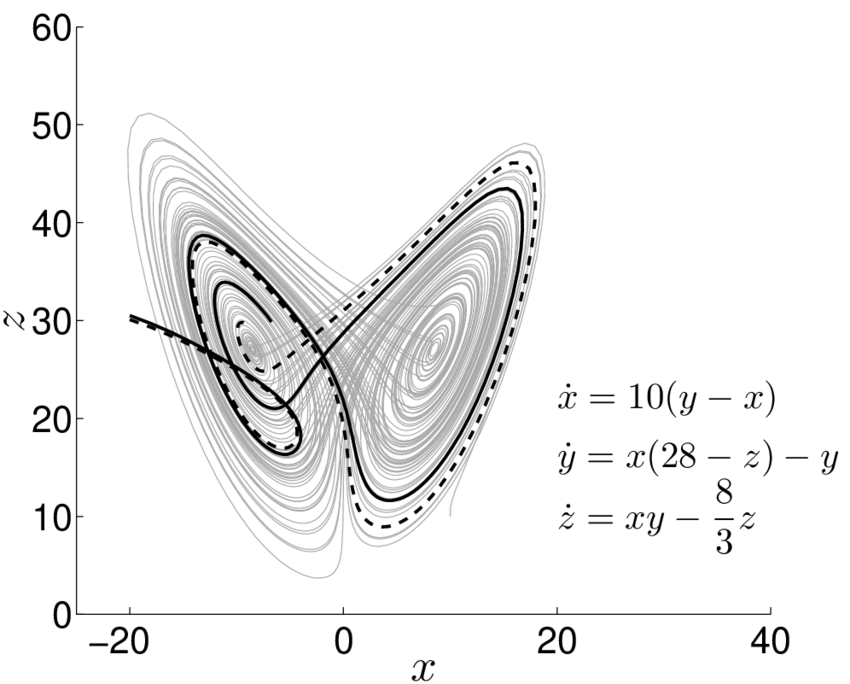
\includegraphics[scale=0.4]{img.png}

\bibliographystyle{plain}
\bibliography{bibfile}

\end{document}